\documentclass{ieeeaccess}
\usepackage{cite}
\usepackage{amsmath,amssymb,amsfonts}
\usepackage{algorithmic}
\usepackage{graphicx}
\usepackage{textcomp}
\usepackage[utf8]{inputenc}
\usepackage{hyperref}
\usepackage{booktabs}

\begin{document}

\title{Electricity Consumption Prediction}
\author{
    \IEEEauthorblockN{González, S. Miguel}, 
    \IEEEauthorblockN{Silva, L. Eric}, 
    \IEEEauthorblockN{Quevedo R. Edson}, 
    \IEEEauthorblockN{Guzmán M. Brian}, 
    \IEEEauthorblockN{Rivera L. Jaime} \\
    \IEEEauthorblockA{\textit{Master's Program in Computer Engineering\\
        Universidad Andrés Bello (UNAB), Chile \\
        MSI608 --- Special Topics in Data Science}}
}

\markboth
{González, Silva, Quevedo, Guzmán y Rivera \headeretal: Electricity Consumption Prediction}
{González, Silva, Quevedo, Guzmán y Rivera \headeretal: Electricity Consumption Prediction}



\begin{abstract}
Electricity consumption forecasting is essential for energy planning and efficient demand management. This study evaluates predictive models for a univariate time series of aggregated daily electricity consumption. The dataset comprises 1,461 consecutive observations from January 1, 2018, to December 31, 2021, with no missing values, duplicate records, or absent dates. Three approaches were compared: a seasonal naive baseline, a seasonal autoregressive integrated moving average (SARIMA) model, and a multilayer perceptron (MLP) optimized through automated hyperparameter search. Models were trained on data from 2018--2020 and evaluated on 365 observations from 2021. SARIMA achieved the best predictive performance, with an MAE of 9.75, RMSE of 12.98, MAPE of 6.72\%, and $R^2$ of 0.852. These results indicate that, for a moderately sized univariate daily series, a statistical model that explicitly represents weekly seasonality can outperform an optimized neural network. Finally, annual Fourier terms were incorporated into a SARIMAX extension to generate an exploratory forecast for 2022.
\end{abstract}

\begin{IEEEkeywords}
Aggregated daily time series, electricity consumption forecasting, multilayer perceptron, SARIMA, seasonal naive model.
\end{IEEEkeywords}

\titlepgskip=-15pt
\doi{}
\maketitle

\section{Introduction}
\label{sec:introduction}
\subsection{Background and Motivation}
\PARstart{E}{lectricity} consumption forecasting is fundamental for supporting energy planning, resource allocation, and demand management. However, the appropriate modeling strategy depends on the temporal resolution and structure of the available information. The dataset considered in this study consists of a single univariate time series of aggregated daily electricity consumption covering four complete calendar years. This setting defines an endogenous forecasting problem in which predictive information must be extracted exclusively from the historical behavior of the series. Preliminary analysis revealed temporal persistence, non-stationarity, weekly seasonality, and longer-term variation associated with the annual cycle. Accordingly, this work investigates whether a statistical model specifically designed for seasonal time series can outperform both a seasonal baseline and an optimized neural network when the available training sample is moderate in size.

\subsection{Objectives}
The primary objective of this work is to develop and evaluate models capable of forecasting aggregated daily electricity consumption from its historical behavior. To achieve this overarching goal, the following specific objectives were established:
\begin{enumerate}
\item Assess the completeness, correctness, distribution, and presence of outliers in the historical electricity consumption dataset.
\item Identify trend, stationarity, autocorrelation, and weekly seasonal patterns in the daily time series.
\item Compare a seasonal naive baseline, a SARIMA model, and an MLP neural network under a chronological evaluation design.
\item Evaluate predictive performance using MAE, RMSE, MAPE, and $R^2$, and analyze daily forecasts together with weekly, monthly, and annual aggregations.
\item Select the best-performing model and generate an exploratory forecast of daily electricity consumption for 2022.
\end{enumerate}

\section{Related Work}
\label{sec:Related Work}
Short-term electricity load forecasting (STLF) has been an active area of research for several decades, with a growing body of literature that reflects the transition from classical statistical methods toward data-driven machine learning and deep learning approaches \cite{ref1,ref2,ref3}. This section reviews the state of the art, contrasting traditional statistical models with modern machine learning techniques and discussing the influence of temporal feature engineering on forecasting accuracy for aggregate system-level electricity demand.

\subsection{Traditional Statistical Approaches}
Early STLF methods relied primarily on linear time series models. Autoregressive integrated moving average (ARIMA), seasonal ARIMA (SARIMA), and exponential smoothing gained widespread adoption due to their simplicity and interpretability, particularly for aggregate system-level demand characterized by strong seasonality \cite{ref7}. These models remain useful as strong baselines, but their linear assumptions limit their capacity to capture the highly non-linear, volatile consumption patterns observed in modern grids \cite{ref1,ref10}. Hybrid strategies that combine traditional time series decomposition with external regressors have been proposed to mitigate these limitations, yet they often require manual tuning and domain expertise that hinder their scalability \cite{ref7,ref11}.

\subsection{Machine Learning Approaches}
Machine learning methods have largely addressed the non-linearity limitations of classical models. Ensemble techniques such as Random Forest and gradient boosting, as well as kernel-based methods such as Support Vector Machines, have demonstrated superior accuracy in short-term demand forecasting compared with statistical baselines \cite{ref7,ref8,ref12}. A recurring finding in the literature is that model performance depends on temporal variability, forecast horizon, and the availability of informative predictors \cite{ref1,ref8}. For daily series, calendar variables such as the day of the week and month, together with lagged consumption values, provide a coherent representation of recurring patterns \cite{ref8,ref12}. This evidence supports the endogenous daily forecasting strategy adopted in the present study.

\subsection{Deep Learning Approaches}
More recently, deep learning architectures have become the dominant paradigm for load forecasting. Recurrent neural networks, particularly Long Short-Term Memory (LSTM) networks, have proven highly effective at capturing long-range temporal dependencies in energy time series \cite{ref8,ref10}. Multiple comparative studies report that LSTM-based models outperform Support Vector Machines and feed-forward neural networks for both aggregated and household-level consumption \cite{ref9,ref10}. More advanced attention-based architectures, including the Temporal Fusion Transformer (TFT), have been introduced to integrate multiple data sources and produce probabilistic forecasts across different forecasting horizons \cite{ref5}. While such models offer interpretability benefits and strong performance, their gains over well-tuned LSTM baselines are not always consistent, particularly for day-ahead horizons \cite{ref5}.

\subsection{Temporal Resolution and Forecast Granularity}
Temporal resolution is a central consideration in short-term load forecasting because it determines which demand patterns can be represented and which model structures are appropriate \cite{ref1,ref4}. Daily aggregate forecasting summarizes system-wide consumption in a single chronological series, emphasizing weekly recurrence, medium-term variation, and annual seasonality. Previous studies show that forecast accuracy depends strongly on matching the model, lag structure, and validation design to the temporal resolution of the observations \cite{ref5,ref11}. Accordingly, the present study evaluates statistical and neural approaches under a consistent daily forecasting framework.

\subsection{Gaps and Positioning}
Despite these advances, several challenges persist. Many forecasting approaches rely on exogenous variables, particularly meteorological information, that may be unavailable or unreliable in practice \cite{ref4,ref6}. Accuracy can also deteriorate during holidays, extreme weather, or other anomalous periods because models depend heavily on historical regularities \cite{ref5,ref11}. Furthermore, comparative evidence for purely endogenous daily consumption forecasting remains limited. This study addresses that gap by evaluating Seasonal Naive, SARIMA, and MLP models on the same chronological train-test partition, thereby providing a reproducible comparison and a basis for future extensions with climate and calendar variables.


\section{Methodology}
\label{sec:methodology}
\subsection{Dataset Description}
The dataset employed in this study consists of a historical record of daily aggregated electricity consumption, with continuous temporal coverage from January 1, 2018, to December 31, 2021, totaling 1,461 consecutive observations (four complete calendar years, including two leap years). Each record contains the year, month, day, and total consumption recorded for the corresponding date. Once the temporal variables are combined into a daily timestamp, the data form a single univariate time series representing aggregate electricity demand. A preliminary structural verification confirmed that the series contains no duplicate records, null values, or missing dates, preserving a complete daily frequency throughout the study period (the quantitative detail of this verification is reported in Section III-B).

\Figure[t!](topskip=0pt, botskip=0pt, midskip=0pt)[width=\textwidth]{figures/fig_daily_series.png}
{Daily aggregated electricity consumption series (2018--2021).\label{fig_daily_series}}

\subsection{Exploratory Data Analysis and Preprocessing}
Prior to modeling, a systematic data quality assessment was conducted along three dimensions: completeness, correctness, and the presence of outliers. Regarding completeness, the complete absence of null values was verified (0 missing records), and the series' temporal index was cross-checked against an artificially generated daily date range covering the entire 2018--2021 period, revealing no discontinuities (0 missing dates out of 1,461 expected). Regarding correctness, the absence of duplicate records and of non-positive or physically invalid values for an electricity consumption variable was confirmed, with a plausible value range between 32.79 and 250.55 units.

For outlier detection, the interquartile range (IQR) criterion was applied, defining as anomalous any observation falling outside the interval $[Q1 - 1.5\cdot IQR,\ Q3 + 1.5\cdot IQR]$; under this criterion, only 2 anomalous observations were identified out of 1,461 (0.14\% of the total), a marginal proportion that did not warrant corrective treatment (imputation or removal); these values were retained in the analysis, as they may correspond to genuine extreme-consumption events rather than sensor errors.

\begin{figure}[t]
\centering
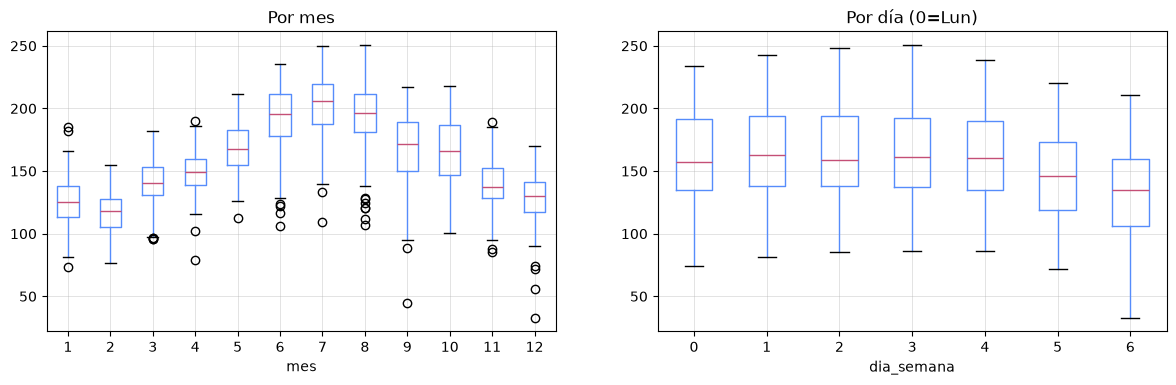
\includegraphics[width=1\linewidth]{figures/fig_outlier_boxplots.png}
\caption{Boxplots of daily consumption by month and by day of week.}
\label{fig:boxplots}
\end{figure}

As a precautionary measure for the modeling stage, a forward-fill step was additionally incorporated into the series, a standard time-series practice to ensure robustness against potential future discontinuities, even though the completeness analysis confirmed that no gaps requiring such treatment existed in the current dataset.
\newline
\begin{figure}[t]
\centering
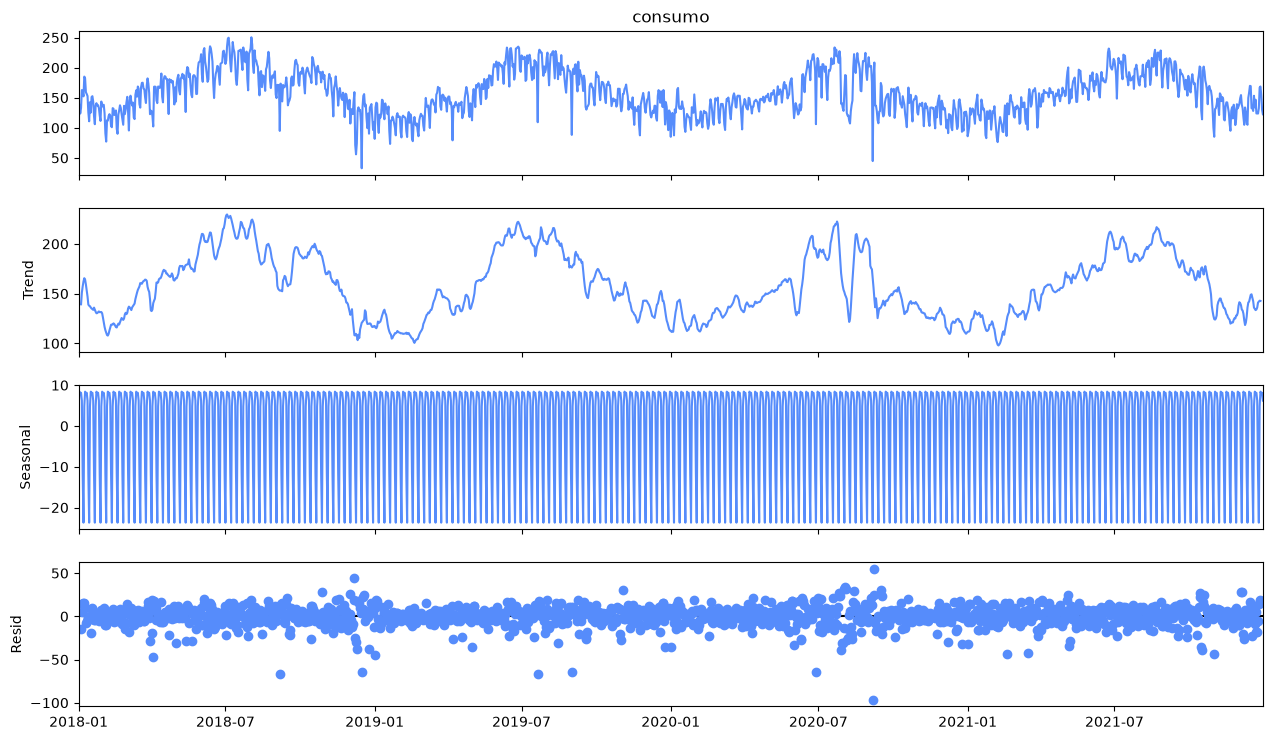
\includegraphics[width=1\linewidth]{figures/fig_seasonal_decomp.png}
\caption{Additive decomposition of the daily series (period = 7).}
\label{fig:fig_seasonal_decomp}
\end{figure}


The exploratory analysis was further complemented by an examination of the series' stochastic properties. The Augmented Dickey-Fuller (ADF) test applied to the original series yielded an ADF statistic of $-2.508$ ($p = 0.1136$), failing to reject the null hypothesis of non-stationarity at the conventional 0.05 significance level. After applying first-order differencing, the ADF statistic decreased to $-11.759$ ($p < 0.0001$), decisively rejecting non-stationarity. This result statistically justifies the use of a differencing order of $d=1$ in the subsequent SARIMA model configuration (Section III-D). In addition, seasonal decomposition (additive model, period = 7) and the analysis of the autocorrelation function (ACF) and partial autocorrelation function (PACF) revealed a clearly defined weekly seasonal pattern --- consistent with the structural difference between weekdays and weekends characteristic of electricity consumption --- along with a longer-period (annual) trend and cyclical component visible in the observed series.

\begin{figure}[t]
\centering
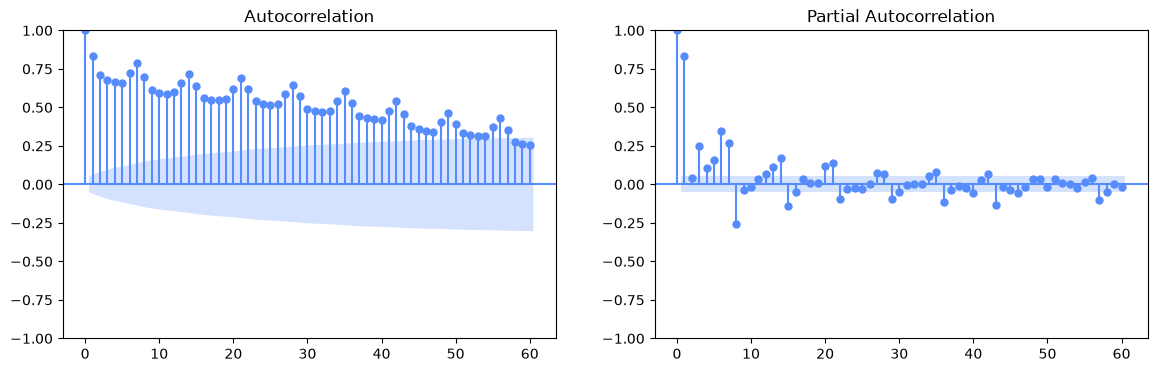
\includegraphics[width=1\linewidth]{figures/fig_acf_pacf.png}
\caption{ACF and PACF of the daily consumption series.}
\label{fig:fig_acf_pacf}
\end{figure}

\subsection{Feature Engineering}
\label{sec:feature engineering}
Given the strictly univariate, daily-granularity nature of the dataset, the feature construction strategy was designed to capture the series' temporal dependence through two complementary mechanisms, each associated wit a different model. First, for the neural network model (MLP), an autoregressive sliding-window variable was constructed: each input observation consists of the 14 immediately preceding consumption values (WINDOW = 14), transforming the forecasting problem into a standard supervised regression task, where the input vector summarizes recent demand behavior and the scalar output corresponds to the following day's consumption. Second, for the SARIMA statistical model, the weekly seasonality --- previously identified through the ACF/PACF analysis (Section III-B) --- is not incorporated as an explicit variable, but is instead natively encapsulated within the model's seasonal component specification ($m=7$), leveraging SARIMA's ability to model such periodicity through its own seasonal autoregressive and moving-average parameters, without requiring external feature engineering. Additionally, for the future forecasting stage (outside the scope of the model comparison in Section IV), annual Fourier exogenous variables were incorporated (365.25-day period, 4 harmonics), in order to capture the long-term seasonal component that SARIMA(2,1,2)(1,0,1,7) alone cannot represent when projecting extended horizons.

\Figure[t!](topskip=0pt, botskip=0pt, midskip=0pt)[width=\textwidth]{figures/fig1_pipeline.jpeg}
{Predictive pipeline architecture (Dataset A --- daily aggregated electricity consumption).\label{fig1_pipeline}}

\subsection{Predictive Modeling}
The dataset partition strictly preserved the chronological order of the series, using the 2018--2020 period as the training set (1,096 observations) and the full 2021 year as the test set (365 observations), thereby avoiding any backward data leakage that a random split would have introduced --- a standard criterion in time-series model validation. Three modeling approaches of increasing complexity were trained and compared over this partition, deliberately selected to quantify the actual performance gain of each level of sophistication:

\begin{enumerate}
\item \textbf{Baseline model (seasonal naive):} predicts each day's consumption as the value observed exactly 7 days earlier, exploiting the weekly seasonality identified during the EDA. Its sole purpose is to serve as a minimum performance threshold: any more complex model must outperform it to justify its additional computational and interpretive cost.
\item \textbf{SARIMA(2,1,2)(1,0,1,7):} a classical time-series statistical model, whose order was selected based on empirical evidence from the ACF/PACF analysis (Section III-B) and the ADF test, which justified a differencing order of $d=1$ and a seasonal component of period $m=7$. Prediction on the test set was performed one step ahead, iteratively incorporating each real test observation via the \texttt{statsmodels} \texttt{append(refit=False)} method, without re-fitting the model's parameters at each step --- this ensures a fair comparison against the MLP, which likewise predicts one day at a time from real recent context.
\item \textbf{Multilayer Perceptron (MLP) neural network:} a supervised learning model that receives the 14-day autoregressive window (Section III-C) as input and produces the following day's consumption as output. The architecture (number of hidden layers $\in \{1,2,3\}$, neurons per layer $\in \{32,64,128,256\}$, and learning rate $\in \{10^{-2},10^{-3},10^{-4}\}$) was not fixed arbitrarily, but determined through automated hyperparameter search (\texttt{keras-tuner}, Random Search strategy, 8 combinations evaluated on a 15\% validation split of the training set), resulting in an optimal architecture of 3 hidden layers of 256 neurons each, with a learning rate of 0.0001. Final training was run for a maximum of 80 epochs with a batch size of 64, incorporating early stopping (patience of 15 epochs, best-weight restoration) to prevent overfitting. Input and output variables were standardized using only the training set's mean and standard deviation, avoiding information leakage from the test set into the normalization process.
\end{enumerate}

The entire development was implemented in Python 3.12, using \texttt{statsmodels} for the SARIMA model, TensorFlow/Keras for the MLP, and \texttt{keras-tuner} for hyperparameter optimization, with fixed random seeds (SEED = 121208) across NumPy, Python's standard \texttt{random} library, and TensorFlow, to ensure reproducibility of the reported results.

\subsection{Evaluation Metrics}
To quantify the predictive performance of the models, four standard error metrics for regression and time-series forecasting tasks were employed, selected in a complementary fashion to capture distinct dimensions of error: absolute magnitude, sensitivity to large errors, relative percentage error, and overall goodness of fit. Let $y_i$ denote the observed real value, $\hat{y}_i$ the value predicted by the model, and $n$ the total number of evaluated observations.

\textbf{Mean Absolute Error (MAE):} quantifies the average error magnitude in the original units of the variable (electricity consumption), without differentially penalizing large versus small errors.

\begin{equation}
MAE = \frac{1}{n}\sum_{i=1}^{n} |y_i - \hat{y}_i|
\end{equation}

\textbf{Root Mean Squared Error (RMSE):} by squaring each error before averaging, it disproportionately penalizes large errors (poorly predicted consumption peaks), relevant in a power grid management context where extreme errors are operationally more costly.

\begin{equation}
RMSE = \sqrt{\frac{1}{n}\sum_{i=1}^{n} (y_i - \hat{y}_i)^2}
\end{equation}

\textbf{Mean Absolute Percentage Error (MAPE):} expresses the error as a percentage relative to the real value, enabling scale-independent performance comparison.

\begin{equation}
MAPE = \frac{100\%}{n}\sum_{i=1}^{n} \left| \frac{y_i - \hat{y}_i}{y_i} \right|
\end{equation}

\textbf{Coefficient of Determination ($R^2$):} measures the proportion of the target variable's variance explained by the model, relative to a trivial model that always predicts the sample mean.

\begin{equation}
R^{2} = 1 - \frac{\sum_{i=1}^{n}(y_i - \hat{y}_i)^2}{\sum_{i=1}^{n}(y_i - \bar{y})^2}, \qquad \bar{y} = \frac{1}{n}\sum_{i=1}^{n} y_i
\end{equation}

The joint use of these four metrics reflects the fact that none is sufficient on its own: MAE and RMSE are expressed in the original consumption units and assess absolute error, whereas MAPE normalizes that error to make it comparable across different aggregation horizons (daily, weekly, monthly, annual); $R^2$, in turn, contextualizes the error against the total variability of the data. It should be noted, as a methodological remark, that computing $R^2$ over the annual aggregation of the test set is mathematically undefined, since the test horizon (2021) corresponds to a single year --- i.e., a single comparison point, insufficient to estimate variance; this case is explicitly reported as not applicable (N/A) in Section IV, rather than being silently omitted.

\section{Results}
\label{sec:results}
The empirical results obtained during the modeling phase show that the daily aggregated electricity consumption series exhibits a strongly seasonal temporal dependence structure, which was effectively captured by the more complex models. Contrary to purely random behavior, consumption exhibits consistent weekly patterns and trend, whose correct modeling translated into substantial reductions in prediction error relative to the baseline.

\begin{figure}[t]
\centering
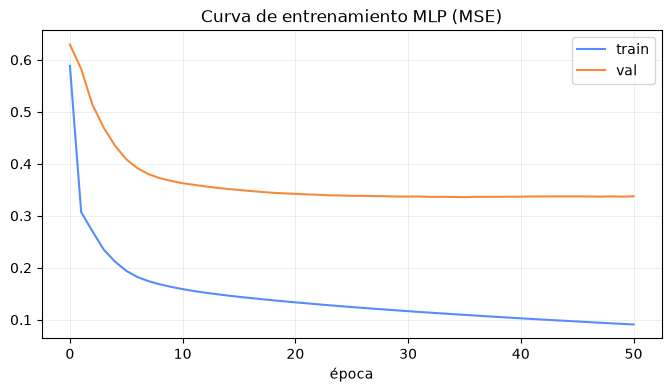
\includegraphics[width=0.78\linewidth]{figures/fig_loss_epochs.png}
\caption{MLP training curve (MSE loss vs. epochs, train and validation).}
\label{fig:loss}
\end{figure}

Table \ref{tab:results_daily} summarizes the performance of the three evaluated models on the test set (year 2021, 365 daily observations), under the four metrics described in Section III-E:

\begin{table}[t]
\centering
\small
\setlength{\tabcolsep}{4pt}
\caption{Model comparison --- daily prediction, 2021 test set}
\label{tab:results_daily}
\begin{tabular}{lrrrrr}
\toprule
\textbf{Model} & \textbf{MSE} & \textbf{RMSE} & \textbf{MAE} & \textbf{MAPE} & \textbf{$R^2$} \\
\midrule
Naive (baseline) & 439.60 & 20.97 & 16.40 & 11.09\% & 0.613 \\
\textbf{SARIMA} & \textbf{168.37} & \textbf{12.98} & \textbf{9.75} & \textbf{6.72\%} & \textbf{0.852} \\
MLP (keras-tuner) & 194.66 & 13.95 & 10.43 & 7.20\% & 0.828 \\
\bottomrule
\end{tabular}
\end{table}


Both advanced models substantially outperformed the naive baseline across all four metrics simultaneously, confirming that weekly seasonality alone (trivially exploited by the baseline) does not capture the full predictive structure of the series. The SARIMA model achieved the best overall performance, reducing RMSE by 41.1\% and MAPE by 39.4\% relative to the baseline, and explaining 85.2\% of the series' total variance ($R^2=0.852$). The MLP, despite being optimized through automated hyperparameter search, performed slightly below SARIMA across all four metrics --- a result consistent with the univariate time-series forecasting literature for moderately sized datasets (1,096 training observations), where classical statistical models with explicit seasonal structure often match or outperform deep learning architectures when the data volume is limited.

Table \ref{tab:results_agg} extends this comparison to the weekly, monthly, and annual aggregation horizons, constructed by summing daily predictions within each period:

\begin{table}[t]
\centering
\scriptsize
\setlength{\tabcolsep}{3pt}
\caption{Aggregated metrics (SARIMA vs. MLP)}
\label{tab:results_agg}
\begin{tabular}{llrrrrr}
\toprule
\textbf{Horizon} & \textbf{Model} & \textbf{MSE} & \textbf{RMSE} & \textbf{MAE} & \textbf{MAPE} & \textbf{$R^2$} \\
\midrule
Weekly & SARIMA & 971.9 & 31.18 & 25.23 & 2.40\% & 0.983 \\
Weekly & MLP & 1035.7 & 32.18 & 25.36 & 2.53\% & 0.982 \\
Monthly & SARIMA & 3500.4 & 59.16 & 51.30 & 1.04\% & 0.996 \\
Monthly & MLP & 6439.9 & 80.25 & 70.22 & 1.52\% & 0.992 \\
Annual & SARIMA & 2153.5 & 46.41 & 46.41 & 0.08\% & N/A* \\
Annual & MLP & 88764.4 & 297.93 & 297.93 & 0.52\% & N/A* \\
\bottomrule
\end{tabular}

\vspace{2pt}
{\footnotesize *Annual $R^2$ is mathematically undefined, since the 2021 test set corresponds to a single year (a single comparison point).}
\end{table}

A notable finding from Table \ref{tab:results_agg} is that MAPE decreases consistently as the temporal aggregation level increases --- from 6.72\% (daily) to 0.08\% (annual) for SARIMA --- a behavior expected in additive time-series forecasting: daily over- and under-estimation errors tend to offset each other when summed within the same period, particularly benefiting the model with lower systematic bias (SARIMA). Fig. \ref{fig:pred_vs_real} illustrates this dynamic visually, overlaying the three prediction curves against the actual observed consumption during the test year: the SARIMA and MLP curves closely track the weekly cycles and medium-term seasonal trend of the real series, while the naive model, although capturing basic weekly periodicity, shows greater dispersion around pronounced consumption peaks and troughs.


\Figure[t!](topskip=0pt, botskip=0pt, midskip=0pt)[width=\textwidth]{figures/fig3_pred_vs_real.png}
{Daily prediction vs. actual consumption on the 2021 test set (Naive, SARIMA, MLP).}

\section{Discussion}
\label{sec:discussion}
One of the findings discussed at greatest length by the team during the project's development relates to the structural nature of each model in relation to the forecasting problem. SARIMA is natively designed for time-series data: its mathematical formulation explicitly incorporates autoregression, differencing, and seasonality components, requiring no additional problem transformation to operate on the series. The MLP, by contrast, required a prior step of problem reformulation: the time series had to be transformed into a tabular supervised learning dataset, using 14-day sliding windows as the input vector and the following day's value as the continuous regression output. This step is neither trivial nor neutral --- it constitutes a conceptual shift from ``modeling a time series'' to ``solving a tabular regression problem that approximates a time series'' --- and helps explain why SARIMA achieved better performance despite the MLP having an architecture optimized through automated hyperparameter search. This result further contrasts with a widespread assumption in much of the recent forecasting literature, which tends to assume that neural network architectures default to outperforming classical statistical models; the results of this study suggest that such an advantage is not automatic and depends heavily on the volume of available data and on whether the problem's seasonal structure can be natively embedded in the model or must instead be empirically learned from the data.

During the exploratory stage, the team also observed that a reliable reading of the autocorrelation (ACF) and partial autocorrelation (PACF) functions required first discarding the series' trend component --- that is, working on the differenced series --- since the long-term trend masked the correlation structure between nearby lags, hindering visual identification of the weekly seasonal pattern. This empirical observation by the team is consistent with, and reinforces, the formal statistical justification provided by the ADF test (Section III-B), which determined a differencing order of $d=1$ to achieve stationarity. Likewise, the inclusion of the seasonal naive model as an additional comparison point --- beyond SARIMA and the MLP --- responded to the need for a broader comparative panorama across modeling paradigms (simple heuristic, classical statistical, and machine learning), allowing the team to quantify not only which model performs best, but how much value each additional layer of complexity actually adds over a trivial solution.

Finally, the team identified during future-forecasting tests that, when projecting horizons beyond one week (7 days), both SARIMA and the MLP tended to generate an illusory stabilization or flattening pattern, losing the ability to represent the series' real medium- and long-term seasonal variability. This behavior is consistent with a known limitation of pure autoregressive models when projecting multiple steps ahead: SARIMA(2,1,2)(1,0,1,7) only captures weekly-period seasonality ($m=7$), and therefore loses reference to the annual seasonality observed in the EDA when extended beyond that horizon. The adopted solution --- incorporating annual Fourier exogenous variables ($K=4$ harmonics) --- allowed this long-term structure, which the model could not infer on its own from purely short-term autoregressive components, to be explicitly injected. It is important to note, however, that this extension into 2022 carries a different epistemological status than the evaluation on the 2021 test set: while the metrics in Section IV are computed against known, real observations, the 2022 forecast constitutes an extrapolation with no available ground truth, and therefore its accuracy cannot be empirically verified with current data --- it should be interpreted as a reasoned projection rather than a validated result.

\section{Conclusion and Future Work}
\label{sec:Conclusion and Future Work}
\subsection{Conclusion}
This study demonstrated that it is possible to accurately predict daily aggregated electricity consumption using time-series and machine learning models trained on historical data, without requiring additional exogenous variables. Among the three approaches compared, the SARIMA(2,1,2)(1,0,1,7) model achieved the best performance (MAPE=6.72\%, $R^2=0.852$ at the daily horizon), outperforming both the seasonal naive baseline and an MLP neural network optimized through automated hyperparameter search. This result confirms that, for moderately sized univariate series with well-defined seasonal structure, classical statistical models with explicit seasonal specification can match or outperform deep learning architectures. It was further observed that the relative error (MAPE) decreases substantially when predictions are aggregated to weekly, monthly, and annual horizons (down to 0.08\% at the annual level for SARIMA), validating the practical usefulness of the proposed framework for energy planning across different time scales, beyond day-to-day operation.

\subsection{Limitations}
This study presents six relevant limitations. First, the use of a system-wide aggregated dataset prevents the capture of localized consumption patterns that would be visible with data disaggregated by substation or region. Second, no exogenous variables such as weather, holidays, or special events were incorporated, factors that likely explain part of the residual error observed across all three models. Third, the model comparison was limited to three approaches (naive, SARIMA, and a single MLP architecture), without evaluating more recent architectures such as LSTMs, Transformers, or ensemble models. Fourth, validation was carried out on a single chronological partition (training 2018--2020, test 2021), without applying rolling-window cross-validation to confirm model performance stability across different periods or anomalous grid events. Fifth, the course material does not specify the exact unit of measurement nor the geographic or institutional origin of the aggregated consumption, which limits the dataset's full traceability. Finally, the extended 2022 forecast constitutes an extrapolation with no ground truth available at the time of this study, and its accuracy therefore cannot be empirically validated against current data.

\subsection{Future Work}
To strengthen the robustness and practical applicability of the proposed framework, future work should focus on the following directions: (1) integration of climatic variables (temperature, humidity, solar radiation) as exogenous inputs, to capture demand peaks associated with heating and cooling loads; (2) expanded algorithmic benchmarking, comparing more advanced deep learning architectures (LSTMs, Transformers) against classical statistical and ensemble models; (3) robust cross-validation through rolling-window time-series techniques, to ensure model stability across different seasons and anomalous grid events; (4) incorporation of calendar-based variables (holidays, long weekends) as additional exogenous inputs, given that electricity consumption often exhibits structural breaks around such dates; and (5) retrospective validation of the 2022 forecast against real data once available, providing a genuine out-of-sample test to quantify the framework's true extrapolation error.

\begingroup
\footnotesize
\setlength{\itemsep}{-2pt}
\begin{thebibliography}{13}

\bibitem{ref1} D. B. Biswal \emph{et al.}, ``Review on smart grid load forecasting for smart energy management using machine learning and deep learning techniques,'' \emph{Energy Reports}, vol. 11, pp. 4702--4723, Jun. 2024.

\bibitem{ref2} H. Eskandari, M. Imani, and M. P. Moghaddam, ``A comprehensive review on deep learning approaches for short-term load forecasting,'' \emph{Renewable and Sustainable Energy Reviews}, vol. 189, art. 114031, Jan. 2024.

\bibitem{ref3} S. Aslam \emph{et al.}, ``A survey on deep learning methods for power load and renewable energy forecasting in smart microgrids,'' \emph{Renewable and Sustainable Energy Reviews}, vol. 144, art. 110992, Jul. 2021.

\bibitem{ref4} A. Rahman, V. Srikumar, and A. D. Smith, ``Predicting electricity consumption for commercial and residential buildings using deep recurrent neural networks,'' \emph{Applied Energy}, vol. 212, pp. 372--385, Feb. 2018, doi: 10.1016/j.apenergy.2017.12.051.

\bibitem{ref5} E. Giacomazzi, K. Hopf, and S. Staake, ``Short-term electricity load forecasting using the Temporal Fusion Transformer: Effect of grid hierarchies and data sources,'' in \emph{Proc. 14th ACM Int. Conf. Future Energy Systems (e-Energy '23)}, Orlando, FL, USA, Jun. 2023, pp. 339--344, doi: 10.1145/3575813.3597345.

\bibitem{ref6} B. Nehme, E. Hajj, and C. Nohra, ``Energy consumption predictions using a neural network,'' \emph{Energy Informatics}, vol. 8, art. 139, Nov. 2025, doi: 10.1186/s42162-025-00601-w.

\bibitem{ref7} N. Sultana, S. M. Z. Hossain, S. H. Almuhaini, and D. Düştegör, ``Bayesian optimization algorithm-based statistical and machine learning approaches for forecasting short-term electricity demand,'' \emph{Energies}, vol. 15, no. 9, art. 3425, 2022.

\bibitem{ref8} S. Bouktif, A. Fiaz, A. Ouni, and M. A. Serhani, ``Multi-sequence LSTM-RNN deep learning and metaheuristics for electric load forecasting,'' \emph{Energies}, vol. 13, no. 2, art. 391, 2020.

\bibitem{ref9} F. M. Fekri, H. Gharib, \emph{et al.}, ``Deep learning for load forecasting: A comparative study,'' \emph{IEEE Access}, vol. 9, pp. 131866--131878, 2021.

\bibitem{ref10} H. Shi, M. Xu, and R. Li, ``Deep learning for household load forecasting---A novel pooling deep RNN,'' \emph{IEEE Transactions on Smart Grid}, vol. 9, no. 5, pp. 5271--5280, Sep. 2018.

\bibitem{ref11} S. B. Taieb, G. Bontempi, A. F. Atiya, and A. Sorjamaa, ``A review and comparison of strategies for multi-step ahead time series forecasting based on the NN5 forecasting competition,'' \emph{Expert Systems with Applications}, vol. 39, no. 8, pp. 7067--7083, Jun. 2012.

\bibitem{ref12} S. Sobhana, S. C. Chowdary, D. Indira, and G. D. Kumar, ``Predicting power consumption of individual household using machine learning algorithms,'' \emph{International Journal on Recent and Innovation Trends in Computing and Communication}, vol. 11, no. 3s, pp. 247--252, Mar. 2023.

\bibitem{ref13} H. Grosan \emph{et al.}, ``Short-Term Load Forecasting: A Comprehensive Review,'' \emph{IEEE Access}, 2024. [Online]. Available: https://ieeexplore.ieee.org/document/10630814

\end{thebibliography}
\endgroup
\EOD
\end{document}
